\documentclass{article}

\usepackage{fancyhdr}
\usepackage{parskip}
\usepackage{amsmath}
\usepackage{wrapfig}
\usepackage{tikz}


\pagestyle{fancy}
\renewcommand{\headrulewidth}{0pt}
\lfoot{Miguel Masó\\miguel.maso@upc.edu}
\rfoot{\today}

\begin{document}

\section*{Natural frequencies of floor slabs}

\begin{wrapfigure}{l}{4cm}
\vspace{-1em}
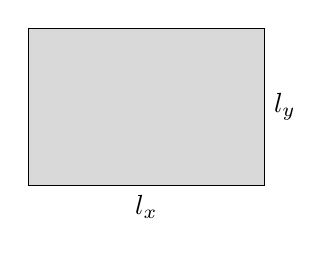
\begin{tikzpicture}
\draw [fill=gray!30] coordinate (O) rectangle (3,2) coordinate (P);
\path (O) -- node [midway,below] {$l_x$} (O -| P);
\path (O -| P) -- node [midway,right] {$l_y$} (P);
\end{tikzpicture}
\end{wrapfigure}

A simply supported rectangular floor of thickness $t$ is considered. The material properties are density $\rho$, Young's modulus $E$ and Poissins's ratio $\nu$. The flexural stiffness is
$$
D = \frac{Et^3}{12(1-\nu^2)}
$$

The frequencies are estimated using the Rayleig's method with an appropriate shape function $\psi$, being $n$ and $m$ the $i^{th}$ mode of vibration for the $x$ and $y$ directions.
$$
\psi = \sin\left(\frac{\pi nx}{l_x}\right) \sin\left(\frac{\pi my}{l_y}\right)
$$

The modal mass is
$$
m_\psi = \int_0^{l_y}\int_0^{l_x} \rho t \psi^2 dxdy
$$

The modal stiffness is
$$
m_\psi = \int_0^{l_y}\int_0^{l_x} D \psi''^2 dxdy
$$

\end{document}